\chapter{Case Study: UAS operating in the NAS}

According to the UAS integration into the NAS roadmap~\cite{nasroadmap} the FAA is working with other government agencies and industry to develop a collaborative UAS modeling and
simulation environment to explore key challenges to UAS integration. The near-term modeling goals are to:
\begin{itemize}
  \item Validate current mitigation proposals
  \item Establish a baseline of end-to-end UAS performance measures
  \item Establish thresholds for safe and efficient introduction of UAS into the NAS
  \item And develop NextGen concepts, including 4-dimensional trajectory utilizing UAS technology
\end{itemize}

We believe that our modeling framework accomplishes each of these goals.  Our modeling framework is extremely flexible allowing it to model a large variety of systems.  We have the ability to detect critical failures.  We have the ability to examine multiple paths through the model and to randomly perturb the model in different ways to explore these paths.  We have the ability to model specific performance measures as extensions to the base model.  While this is left to future work the concept of a set of Actors which can be attached to a third party model to perform performance measuring is very attractive when attempting to standardize model behavior.  We also have the ability to generate human workload metrics which is valuable for setting safety thresholds and analyzing new designs.  We also have the ability to use different levels of abstraction for each portion of our model.  This is ideal while attempting to develop new concepts as it allows us to predict the results of model changes without an exact understanding of how the changes will be implemented.  

The roadmap~\cite{nasroadmap} also identifies several interrelated research challenges:
\begin{itemize}
  \item Effective human-automation interaction (level; trust; and mode awareness)
  \item Pilot-centric ground control station design (displays; sensory deficit and remediation; and sterile cockpit)
  \item Display of traffic/airspace information (separation assurance interface)
  \item Predictability and contingency management (lost link status; lost ATC communication; and ATC workload)
  \item Definition of roles and responsibilities (communication flow among crew, ATC, and flight dispatcher)
  \item System-level issues (NAS-wide human performance requirements)
  \item And airspace users� and providers� qualification and training (crew/ATC skill set, training, certification, and currency)
\end{itemize}

Our modeling framework was specifically designed to model human-automation interaction for UAS.  Our WiSAR model specifically demonstrates predictability and contingency management for each path in the model.  The DiRG allows us to model specific roles and their responsibilities while the DiTG defines communication flow between different roles.  And our workload metrics are ideal for verifying human performance.

Due to the nearly identical nature of the FAAs goals with our own we have decided to demonstrate the recent re-factoring by modeling a basic UAS integrating with the NAS.  Due to our lack of domain knowledge we have had to make a fair number of assumptions in order to achieve a high level of abstraction.  Despite the high level of abstraction we believe that the results are still quite impressive.

\section{Model Scenario and Assumptions}

A UAS plans to operate within the NAS, see figures~\ref{fig:uasnasdirg} and ~\ref{fig:uasnasditg}.  The UAV will take off and land at an airport serving both manned and unmanned aerial vehicles.  The UAV Operator is located at this airport and visually monitors the takeoff and landing of the UAV.  UAV state is continuously shown on the UAS GUI.

There is an FAA system which provides real-time notice to airmen (NOTAM) information.  The UAS connects to this system and displays these NOTAMs on a GUI.  The FAA system also allows UASs to file flight plans.  Filed flight plans are automatically checked for simple conflicts such as crossing NOTAMS or duplicate takeoff/landing times.  If there is a conflict the FAA system flags the flight plan for an ATC (Air Traffic Controller) and displays these requests on its GUI.  The ATC then approves or denies flight plans, using the FAA System GUI, at their leisure.  This approval/denial then becomes available to the UAS which displays it on its GUI.  

The FAA system also provides radar information to the ATC through its GUI.  The ATC uses this information to spot potential collisions with UAVs.  If a potential UAV collision is detected the ATC creates an emergency NOTAM in the region of conflict.  This emergency NOTAM is seen by the UAS.  If the UAV is in or near the emergency NOTAM it must change course to immediately evacuate/avoid the NOTAM.  This can be done automatically by the UAS or manually by the UAV Operator.  Once the UAV has finished avoiding the emergency NOTAM it enters a loiter state.  The UAV Operator is then required to change the flight plan before the UAV will leave the loiter state.  

The UAS also has a radar for the UAV which can detect nearby objects.  This information is displayed on its GUI and if the UAV Operator detects a potential collision they will begin the deconfliction procedure which requires changing the current flight plan.  Once the UAV has landed the scenario is considered complete.

\begin{figure}[h]
\begin{center}
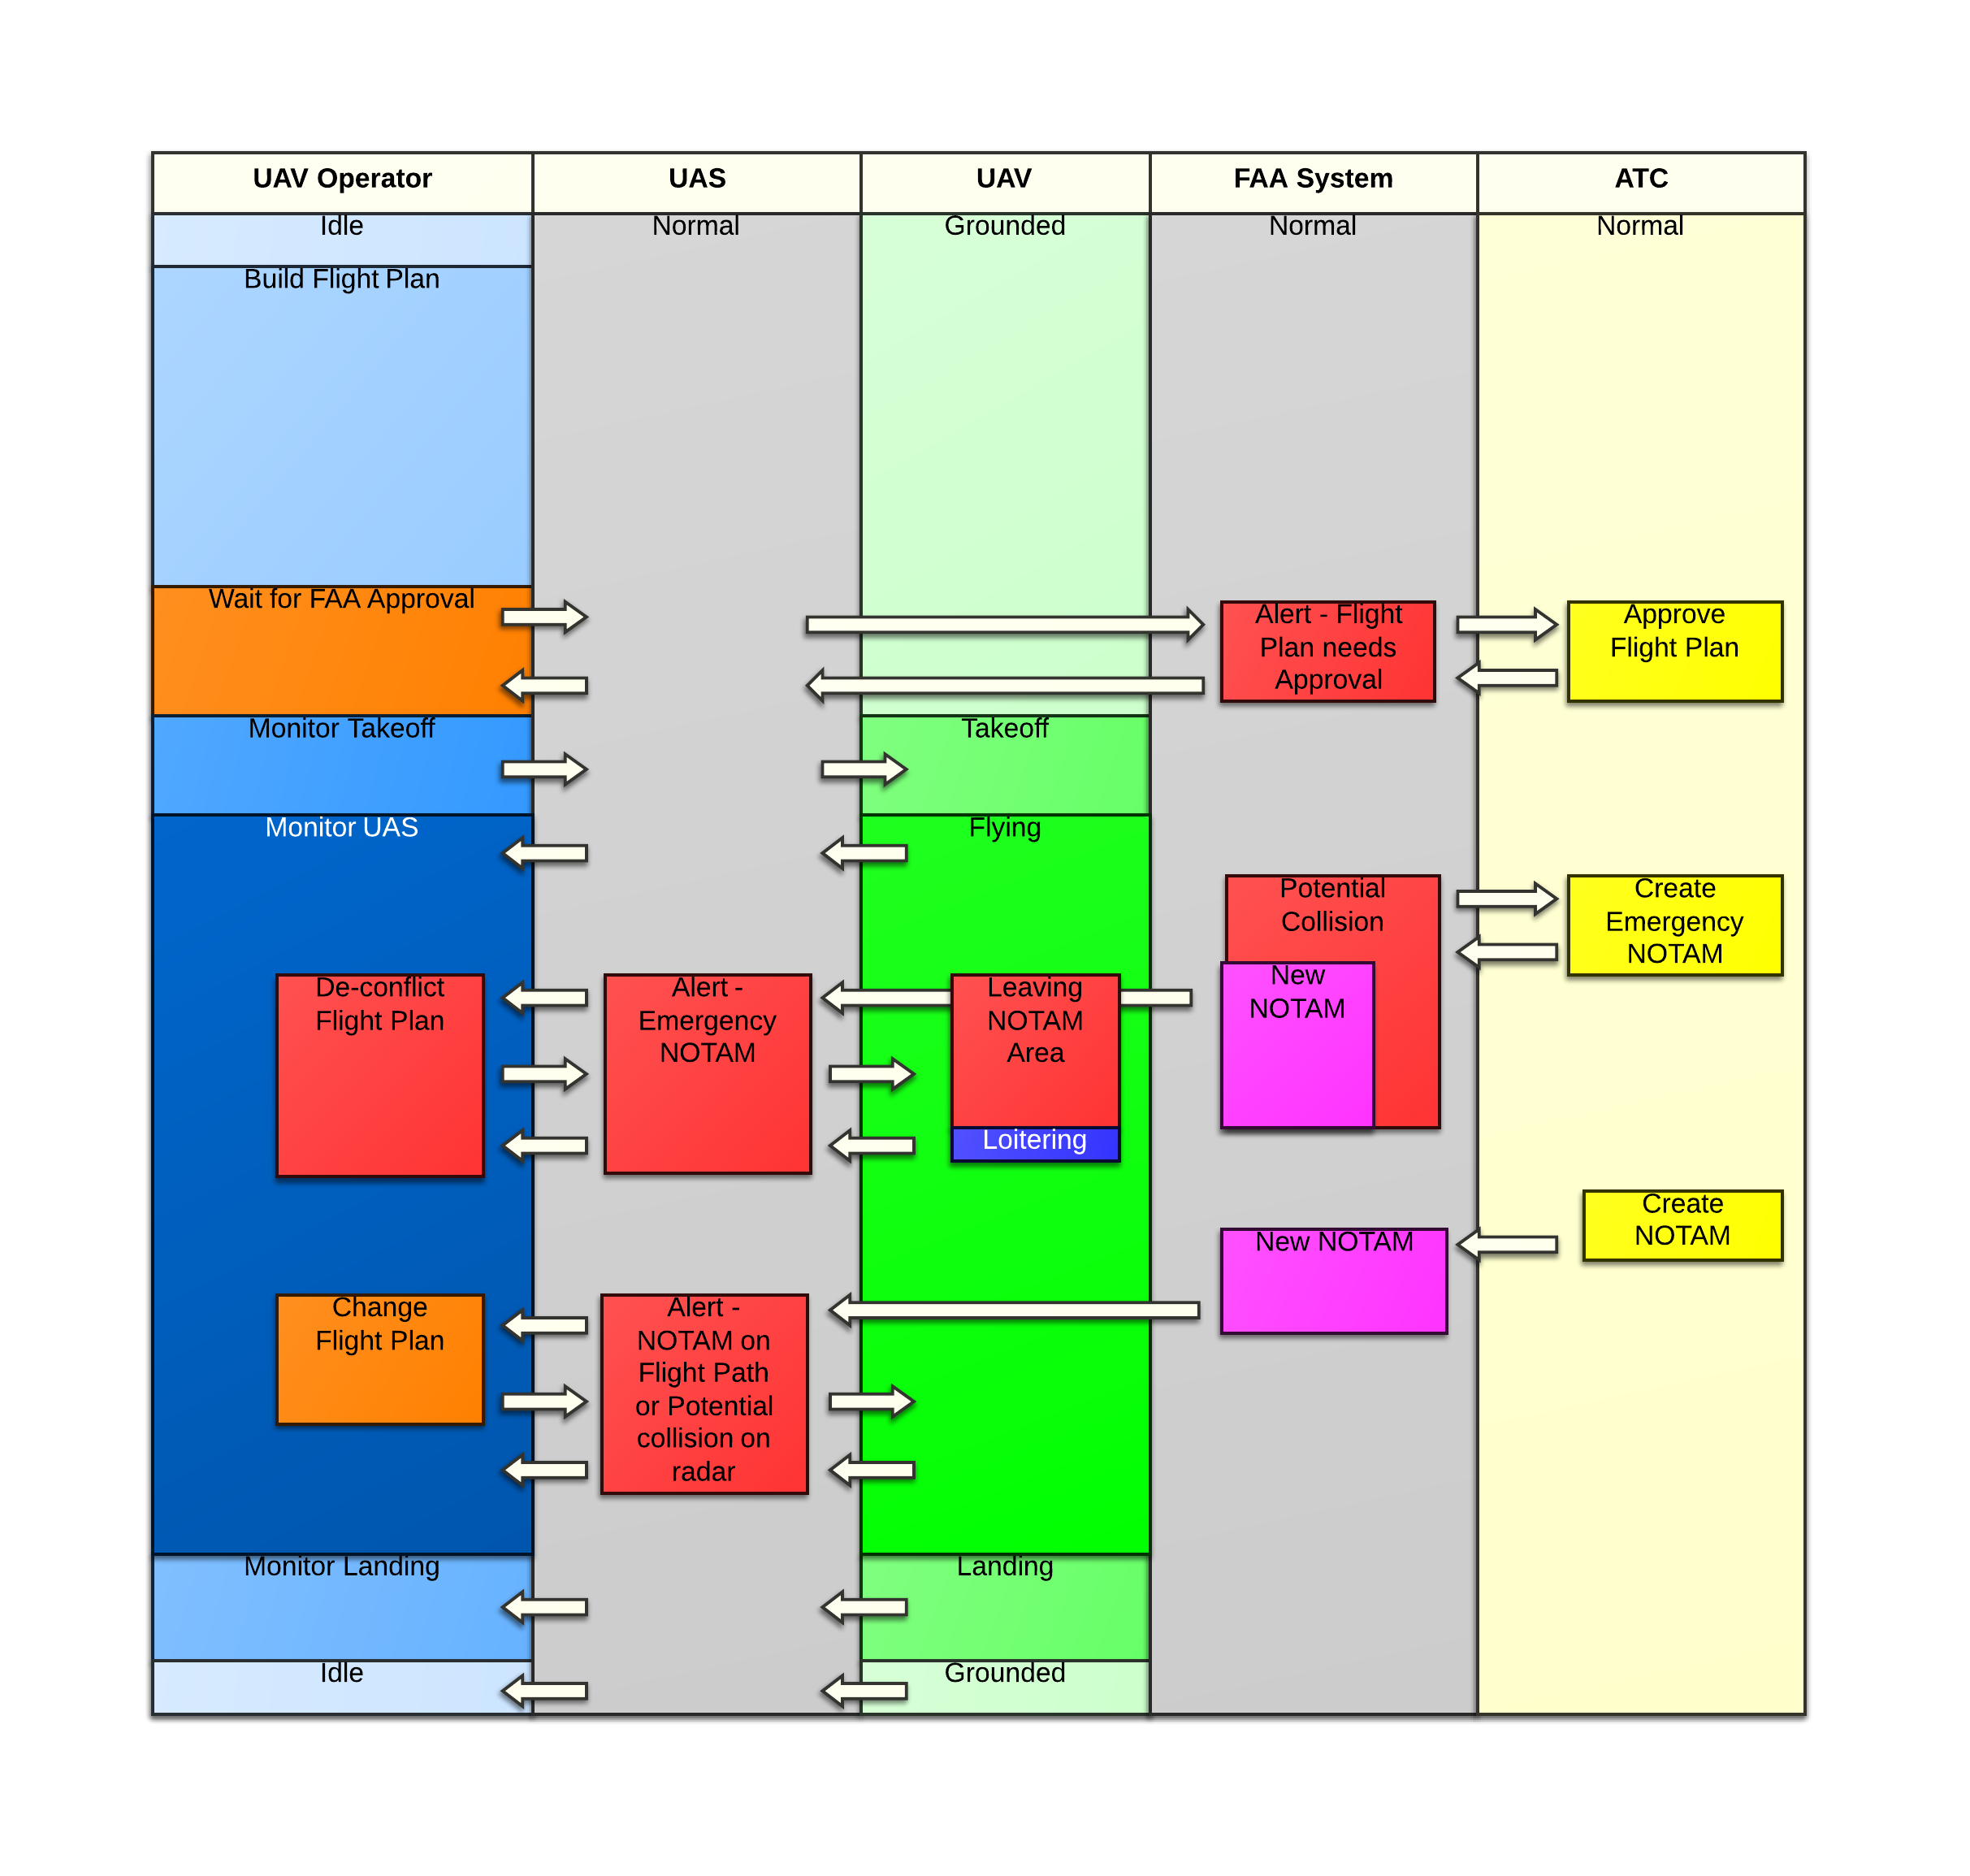
\includegraphics[width=6in]{uasnasdirg.png}
\caption{DiRG: UAS integration into the NAS Model}
\label{fig:uasnasdirg}
\end{center}
\end{figure}

\begin{figure}[h]
\begin{center}
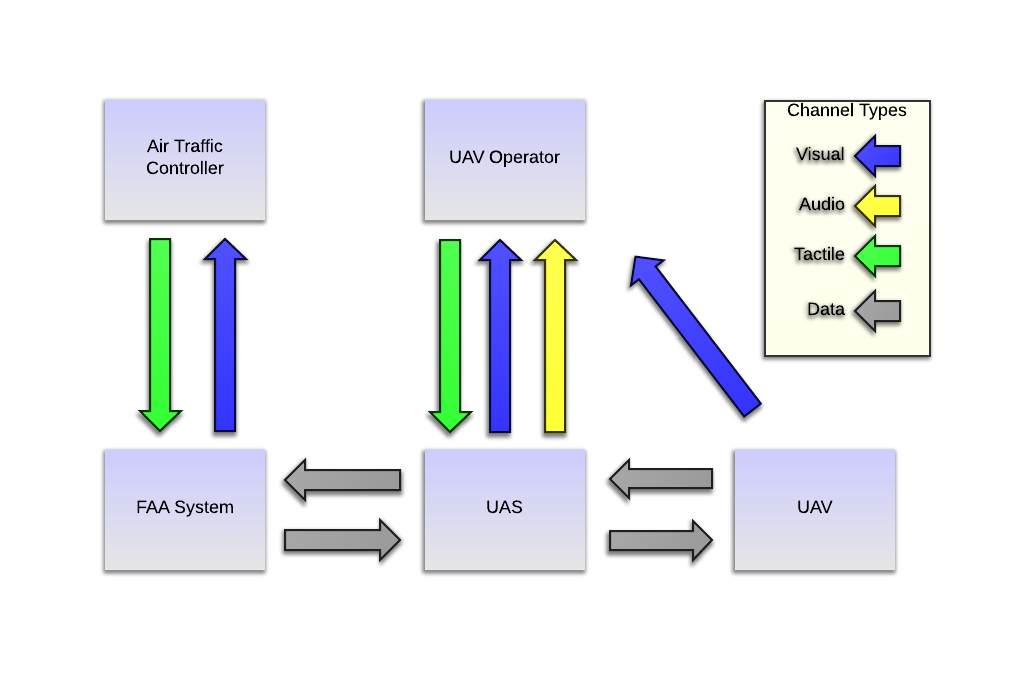
\includegraphics[width=5in]{uasnasditg.png}
\caption{DiTG: UAS integration into the NAS Model}
\label{fig:uasnasditg}
\end{center}
\end{figure}

\subsection{Assumptions}

The number of assumptions made in this scenario is too great to fully list.  Instead we have only attempted to list the major assumptions which are required for the model to perform as designed.
\begin{itemize}
  \item The UAV has an unlimited flight time, never loses contact with the UAS, can takeoff and land without incident, and has accurate GPS data, is non line-of-sight.
  \item The UAS never loses connection to the FAA System, all communication with the UAV and FAA System is instant, no bugs, can create flight plans, can detect NOTAMs on the flight plan, can automatically direct the UAV out of an emergency NOTAM, displays radar information from the UAV.
  \item The UAV Operator detects all warnings displayed on the UAS GUI, generates flight plans which do not touch NOTAMS, can always deconflict the UAV, never gets fatigued.
  \item The FAA System distributes NOTAMS and automatically detects if a flight plan needs to be approved by the ATC.
  \item The ATC detects all information displayed on the FAA System GUI, can add NOTAMS to the FAA System, always adds NOTAMS correctly, approves all flight plans.
\end{itemize}

\section{Building the Model}

Building the model using XML was a very different experience.  In retrospect it would have been valuable to have WiSAR modeled in Java and XML so a direct comparison would be available.  Initially working with a single xml file instead of multiple Java class files was very convenient.  Additionally the ability to validate the model each time we added a new transition led to very rapid development.  Unfortunately as the model complexity increased the added readability, see figure~\ref{fig:read_transition}, was not enough to counter the complexity as the number of transitions and inter-Actor communications increased.  

\begin{figure}[h]
\begin{center}
\subfigure[Java Transition]{
	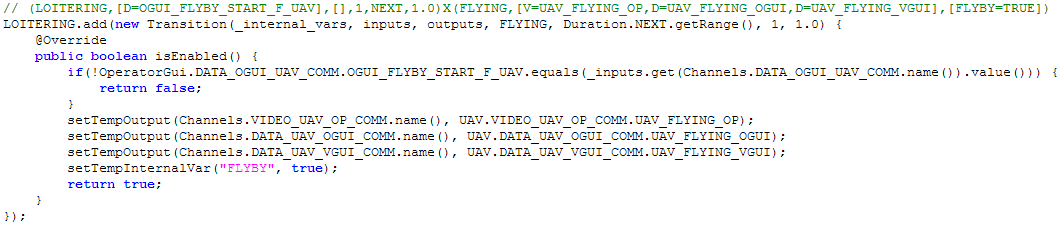
\includegraphics[width=\textwidth]{java_transition.png}
	\label{subfig:subtop}
}
\subfigure[XML Transition]{
	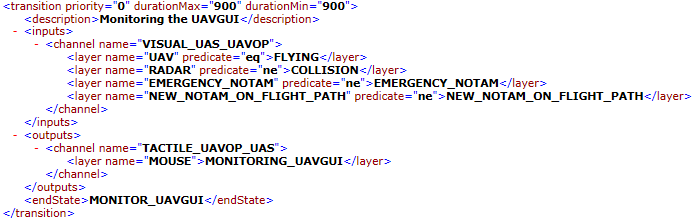
\includegraphics[width=\textwidth]{xml_transition.png}
	\label{subfig:subbot}
}
\caption{Transition Readability Comparison}
\label{fig:read_transition}
\end{center}
\end{figure}

The Enhanced Operator Function Model (EOFM), an XML based modeling language, can be visualized as a tree-like graph due to the way it is structured~\cite{bass2011toward}.  This visualization allows the modeler to see the hierarchical ordering of actions belonging to a task.  Unfortunately the use of XML to format the model did not provide a similar visualization.  In future work it may be valuable to examine a different XML structure which does allow improved visualization of the model.

\subsection{Modeling Approach and Common Errors}

Past experience has shown us that modeling of these complex systems can become very difficult.  In an effort to reduce the complexity we used the following modeling approach.  We first defined each Actor in the system and gave them a starting state.  From here we broke the work into task sequences.  Each task sequence represents the flow of data through the system, initiating from an external event.  For example our model begins with a start mission event which is received by the UAV Operator.  We then implement transitions in sequence until no new transitions are needed.  Each time a new transition is added to the model we run the model to check that the XML is correct and to verify that the new transition is reached.  The full model can be seen in appendix~\ref{XMLModel}.

While this approach was effective it was not a trivial task.  By design the transition sequence moves between Actors requiring the modeler to constantly jump around in the model XML.  Transition sequences will often fork when the action of one Actor causes multiple Actors to respond.  This often results in truncated branches within the model which get forgotten.  One reason for running the model after adding a new transition is that when the complexity causes modeling errors they typically appear in two fashions.  The first is when an Actor becomes trapped in the current state.  This is the more desirable behavior as it is easier to track down.  The second typical error is an infinite loop.  These can be much more difficult to track down.  Infinite loops are often caused by missing transitions, which are normal during model construction.  If the loop is not caused by a missing transition then more in-depth analysis is needed to find the error.  The Java debugger along with the levels of debug output make tracking down these errors rather straight forward, although the process can be time consuming.  While there are many ways to get into an infinite loop we will only mention two common examples.  They are improper transition overriding and uncleared output channels.  Transition overriding happens when you have one transition which is overridden by another before it can fire.  While transition overriding is a desirable behavior, gaps in the transition logic can cause an Actor to continuously cycle between transitions without ever firing a transition and moving to the next state. This can be thought of as undefined behavior.  To fix this, define the behavior for each possible scenario by creating transitions for all combinations of inputs that the Actor cares about.  The simulator will prevent a transition from replacing itself making it better to error on the side of too many transitions.  Uncleared output channels cause an Actor to believe that new input has been received even though it has not sending the Actor into an infinite cycle.  It is often best practice to clear an Actors outputs once those outputs are no longer needed.  If it is important that the input values not be cleared then another approach is to use Actor memory to track changes in input.

While the use of XML to create the model was much more efficient we still feel that a more effective approach to modeling is needed which helps standardize the modeling formats and prevent common errors.  Whether this approach is a different XML structure, an entirely new format, or a GUI interface which helps visualize the data flow and transition sequences we leave to future work.

\section{Model Results}

We were very impressed with the results generated with this new case study which can be seen in figures~\ref{fig:uavop_baseline},~\ref{fig:atc_baseline},~\ref{fig:uavop_manual},~\ref{fig:atc_manual},~\ref{fig:uavop_auto},\ref{fig:atc_auto}, and~\ref{fig:uavop_conflict}  We created three variations of the model.  The first variation involved an uneventful flight.  The second variation involves the UAV Operator manually avoiding an emergency NOTAM.  The third variation involves the UAS automatically avoiding an emergency NOTAM.  The second and third variations also involve a possible UAV collision and the ATC adding a NOTAM onto the UAV flight path.  Additionally we added a fourth variation which involves the UAV Operator being interuped by another person while deconflicting the UAV.  Currently we are only showing the metrics for the human Actors.  For each variation we have four charts depicting the UAV Operator workload and four charts depicting the ATC workload.  The first three charts represent the resource input, resource output, and decision workload.  The last chart shows the combined total workload next to the adapted Wickens workload.  For each chart the y axis represents the workload value while the x axis represents actor state for the given delta time.  What this means is that the x axis cannot be seen as a normal timeline since each time step represents an arbitrary amount of time.  Instead this should be viewed as a progressive change in Actor workload for each time step were a transition was fired.

\subsection{Inter Actor Comparison}

When comparing figures \ref{fig:uavop_baseline} and \ref{fig:atc_baseline} their relationship becomes very clear.  For this scenario the UAV Operator creates a flight plan for his mission.  When he finishes the flight plan he sends it to the FAA System where it is flagged to be approved by the ATC.  The ATC then performs the approval and returns back to normal operations.  The UAV Operator receives the approval and begins normal mission operation which involves a slightly higher workload.  This is reflected beautifully in the Actor workload.  The UAV Operator workload spikes during flight plan creation then flat lines while waiting for a response.  Once he receives the response he spikes again as he performs his mission.  The ATC workload is just the opposite spiking while he is approving the flight plan and returning to normal afterwards.  The comparison of the other variations show the same correlations.  We also see from figure \ref{fig:atc_manual} that the delayed action of the UAV Operator causes the ATC to remain in a high workload state for a long period of time telling us that something is wrong.  By looking at the Actor state we see that the UAV Operator was already in the process of deconflicting the UAV and was not able to immediately respond to the ATC emergency NOTAM.  The last variation shows an improvement in this regard as the UAS automatically diverts the UAV out of the emergency NOTAM while the UAV Operator is busy.  This example demonstrates how the workload modeling allows us to detect problems within the model then analyze fixes to those problems.

\subsection{Intra Actor Comparison}

When comparing figures \ref{fig:uavop_manual} and \ref{fig:uavop_auto} at first glance the metrics appear almost identical.  This is good as these models are nearly identical.  Upon closer examination we see that when the UAV Operator has to manually avoid the emergency NOTAM there is a prolonged increase in resource input workload, an extra spike of resource output workload, and a noticeable spike in decision workload once the UAV Operator begins the process of avoiding the NOTAM.  This results in a significant workload spike compared to the more stable workload seen in the automated emergency NOTAM avoidance.  Another difference which is less noticeable is that the manual emergency NOTAM avoidance takes longer to complete than the auto avoid feature something which is critical in these types of situations.

To make this simple model a little more interesting we decided to add an interruption to the auto avoid variation of the model.  See figure \ref{fig:uavop_conflict}.  When the UAV Operator begins the first deconfliction procedure he is interrupted by another person, a dummy Actor added to the model just for this interruption.  Instead of ignoring this interruption the UAV Operator attempts to communicate with this person while still performing the deconfliction procedure.  This results in a visual channel conflict as the UAV Operator is watching both the UAS GUI and the person who interrupted him.  In addition to this the UAV Operator is now in a high load/multi tasking state.  The result is a workload value of 20 which is almost double the next highest workload value seen in the simulation.  Although this spike in workload has yet to be validated it does match our intuition for the situation.  We would also like to point out how well these results lend themselves to workload thresholds.

While we are mostly pleased with the workload results there are a few anomalies in the results which are misleading.  The most commonly occuring anomaly is a drastic decrease in workload followed immediately be an equally drastic increase in workload.  This tends to happen when an Actor is transitioning into the same state it just left.  The spike happens because we are collecting metrics twice for each step in the delta clock.  Once right before the active transitions are fired and once after they are fired.  

\subsection{Workload Analysis}

We found the chart breakdown to be particularly useful in analyzing the results.  In the resource input workload chart we get an idea of how many channels, layers, and memory objects the Actor is observing.  By comparing this with the resource output workload we can see when the inputs occasioned a response from the Actor.  For the most part these charts are well behaved and follow the workload patterns which we know about.

On the other hand the decision workload typically jumps all over the place.  While we believe the increase in decision workload does in fact increase workload we are unsure how to weight this value in comparison with the resource and temporal workload values.  This is something which needs to be verified through sensitivity and user studies, future work which is important for presenting this modeling framework to the human machine system community.

The last analysis we would like to make is the comparison of our workload metric to that of the adapted Wickens metric.  The general flow of the two metrics is very similar, this is expected since everything in the Wickens metric also exists in our workload metric.  What is more interesting is were the two metrics differ.  Our workload metric is comprised of 9 different values each of which can range from 0 to 2+.  This adds a fair amount of detail into the workload measurement which can be seen by comparing the two values for any of the different model variations.  Where Wickens shows a flat line our metric shows a heart beat which tells us much more about what is causing the additional workload.

\begin{figure}[p]
\begin{center}
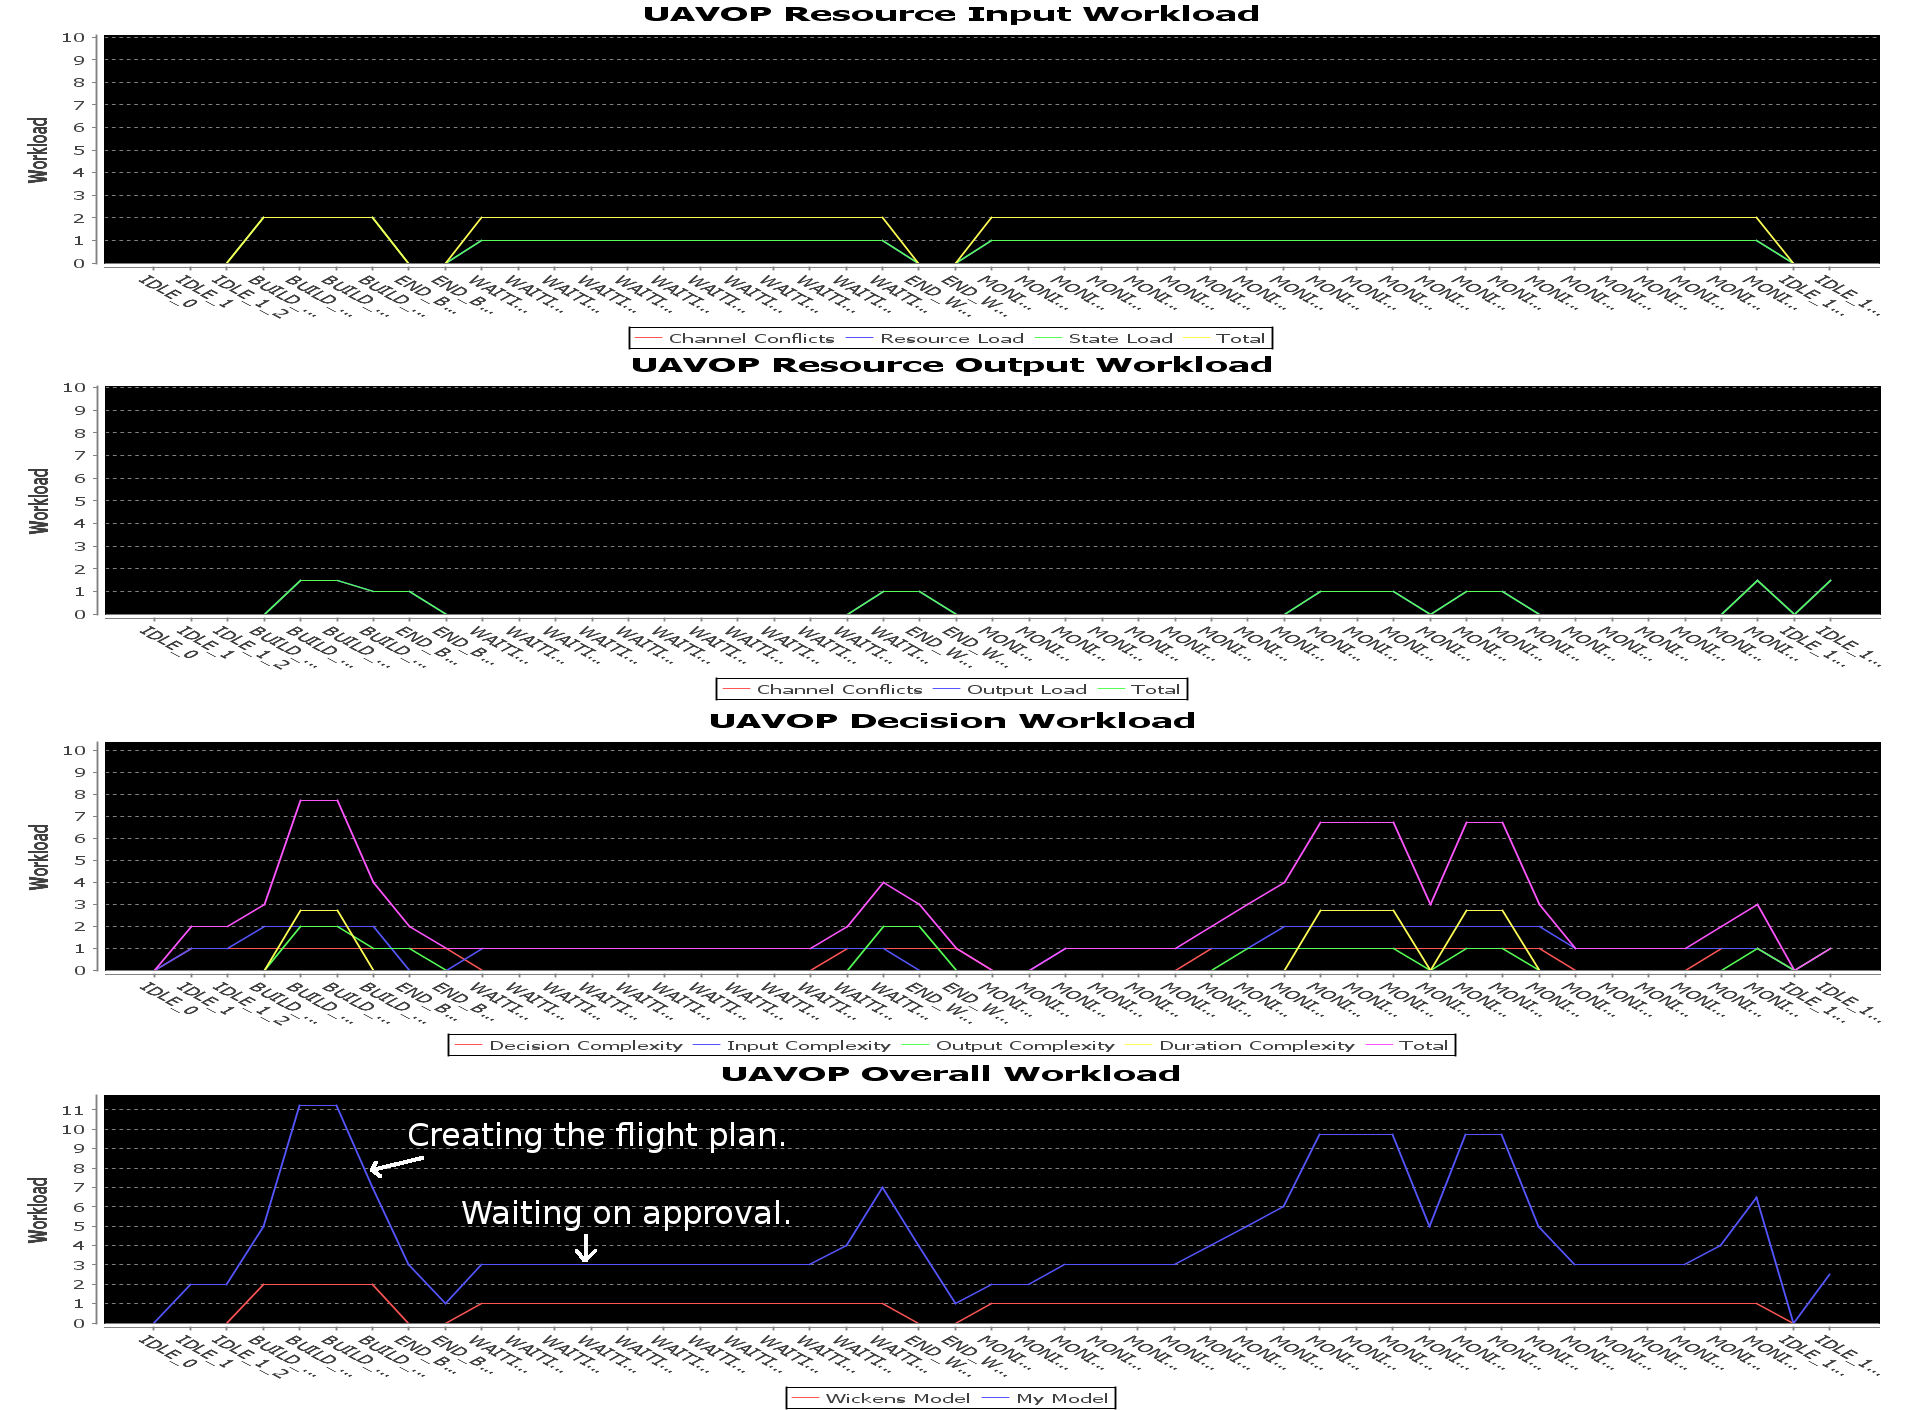
\includegraphics[width=\textwidth,height=\textheight]{UAS_in_NAS_no_events_UAVOP.png}
\caption{UAV Operator: Baseline}
\label{fig:uavop_baseline}
\end{center}
\end{figure}

\begin{figure}[p]
\begin{center}
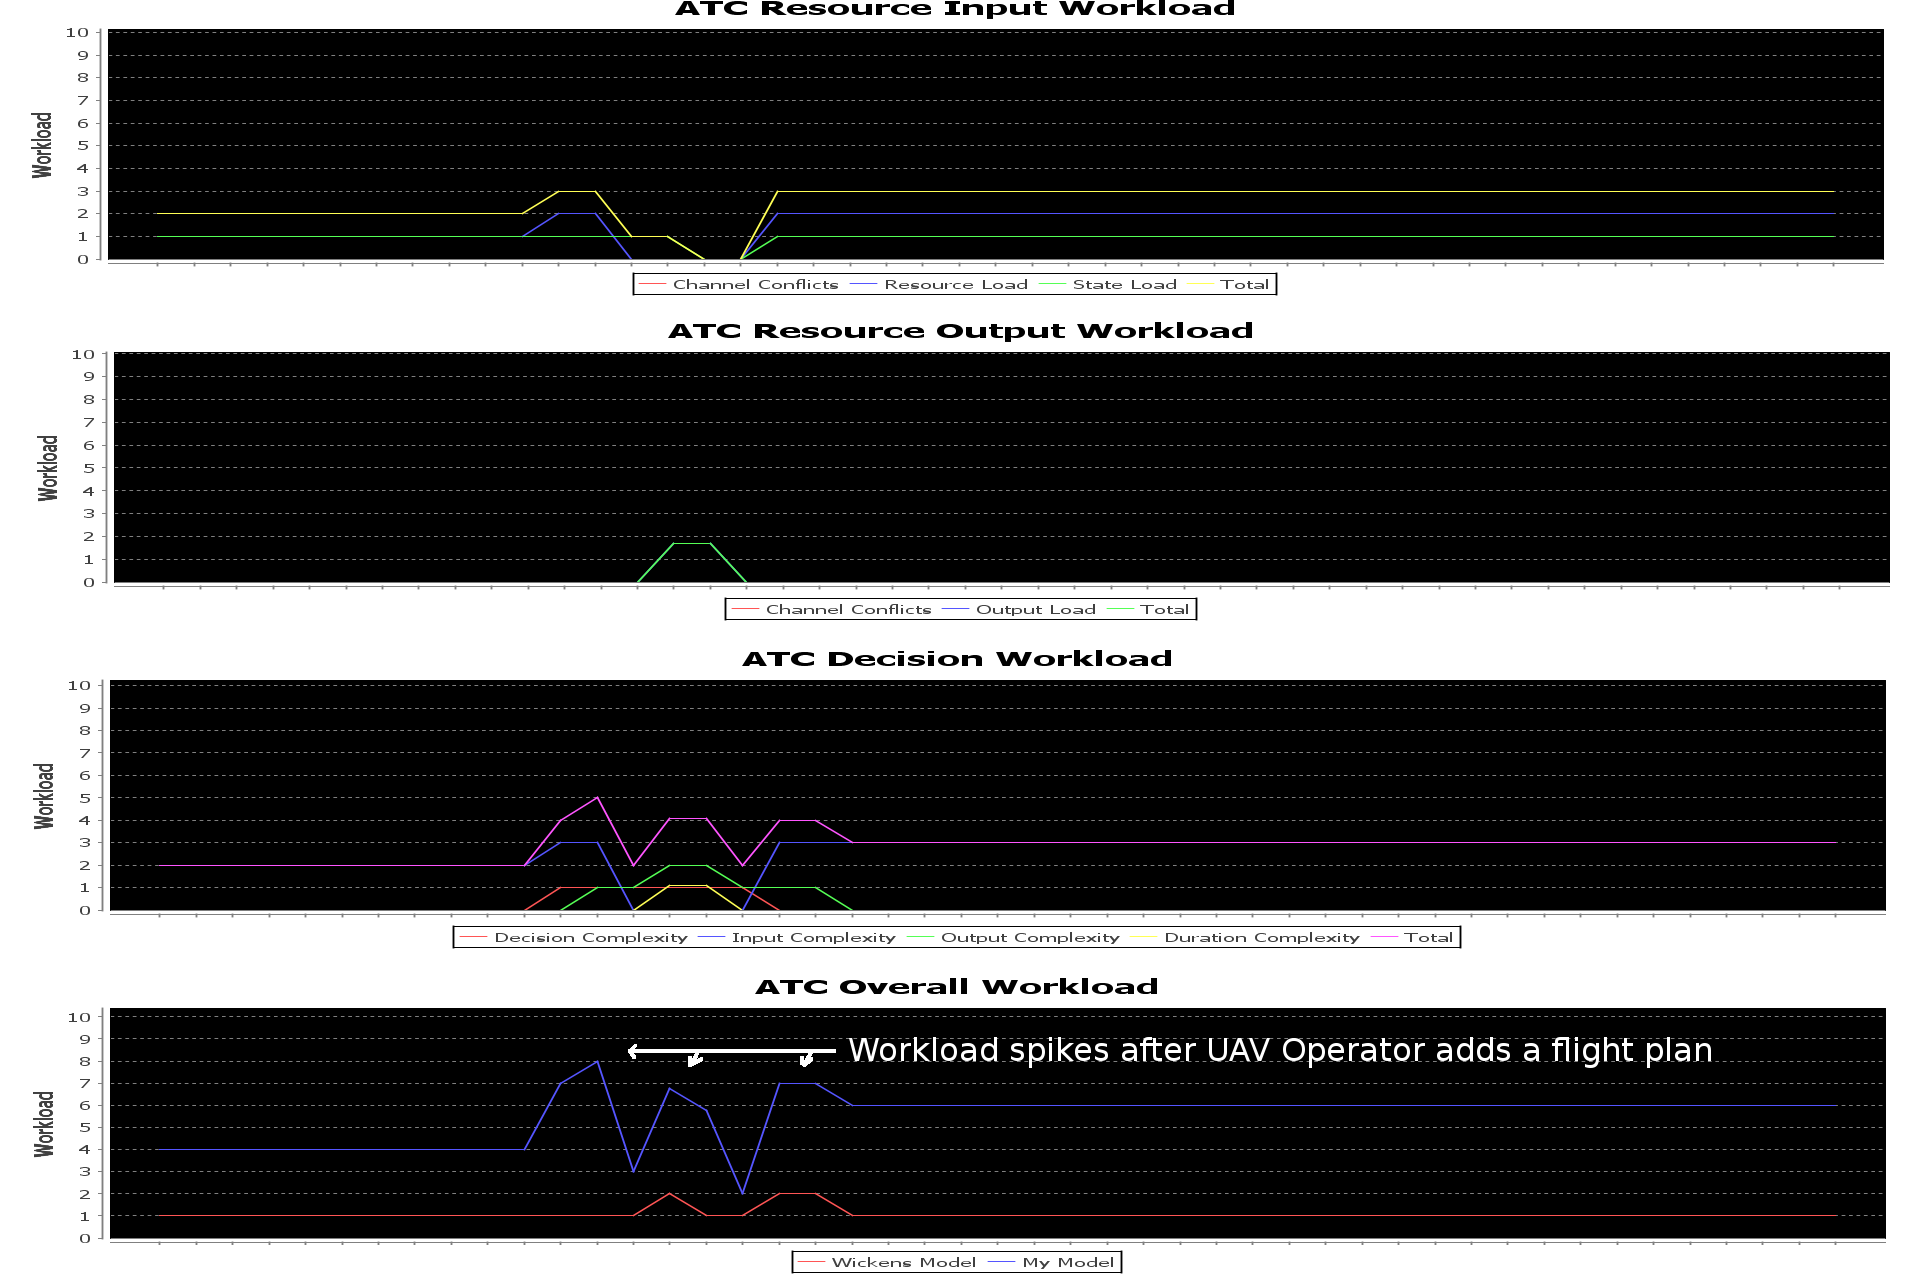
\includegraphics[width=\textwidth,height=\textheight]{UAS_in_NAS_no_events_ATC.png}
\caption{ATC: Baseline}
\label{fig:atc_baseline}
\end{center}
\end{figure}

\begin{figure}[p]
\begin{center}
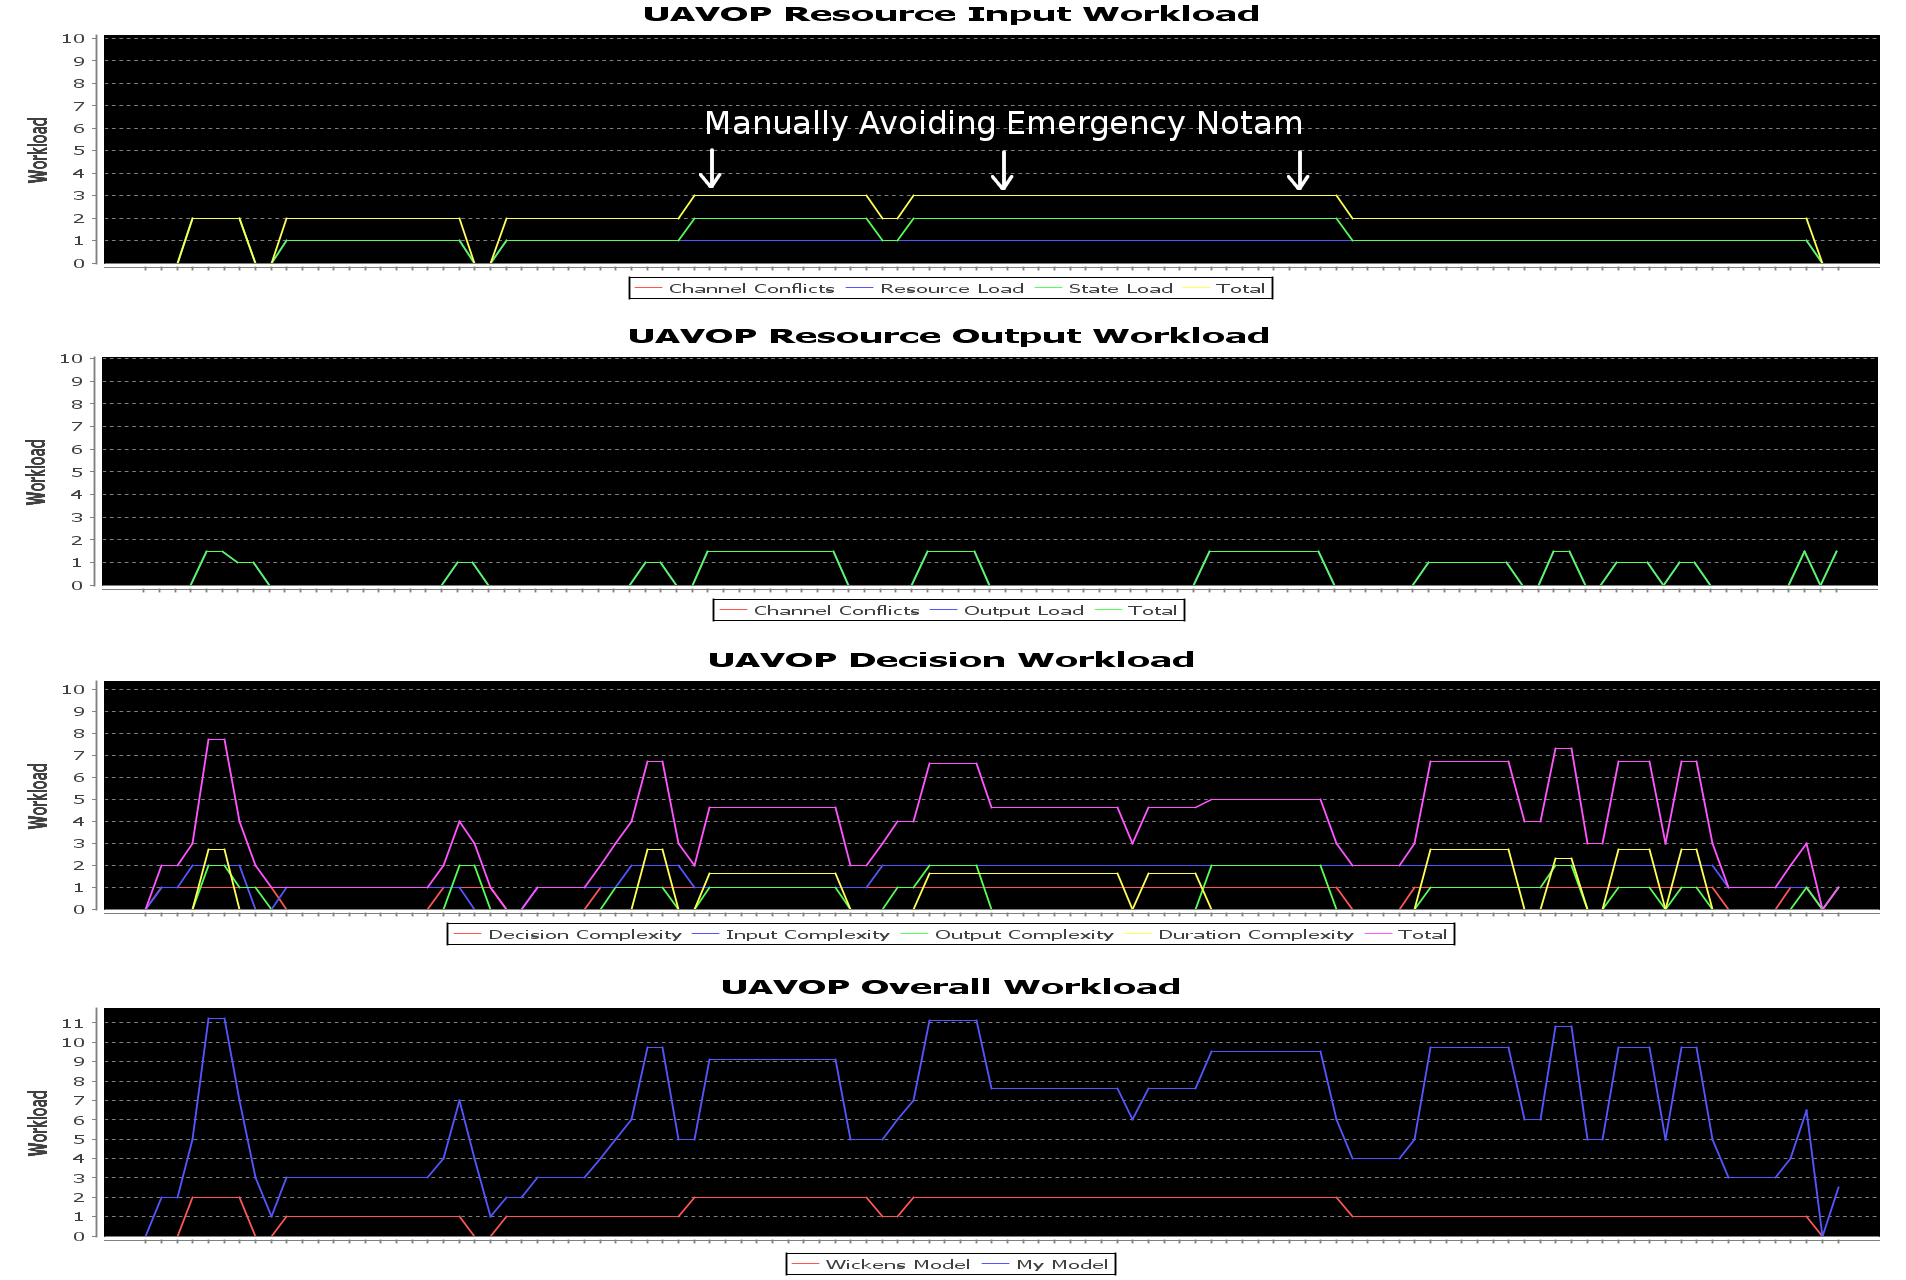
\includegraphics[width=\textwidth,height=\textheight]{UAS_in_NAS_manual_emergency_notam_UAVOP.png}
\caption{UAV Operator: Manually Avoided Emergency NOTAM}
\label{fig:uavop_manual}
\end{center}
\end{figure}

\begin{figure}[p]
\begin{center}
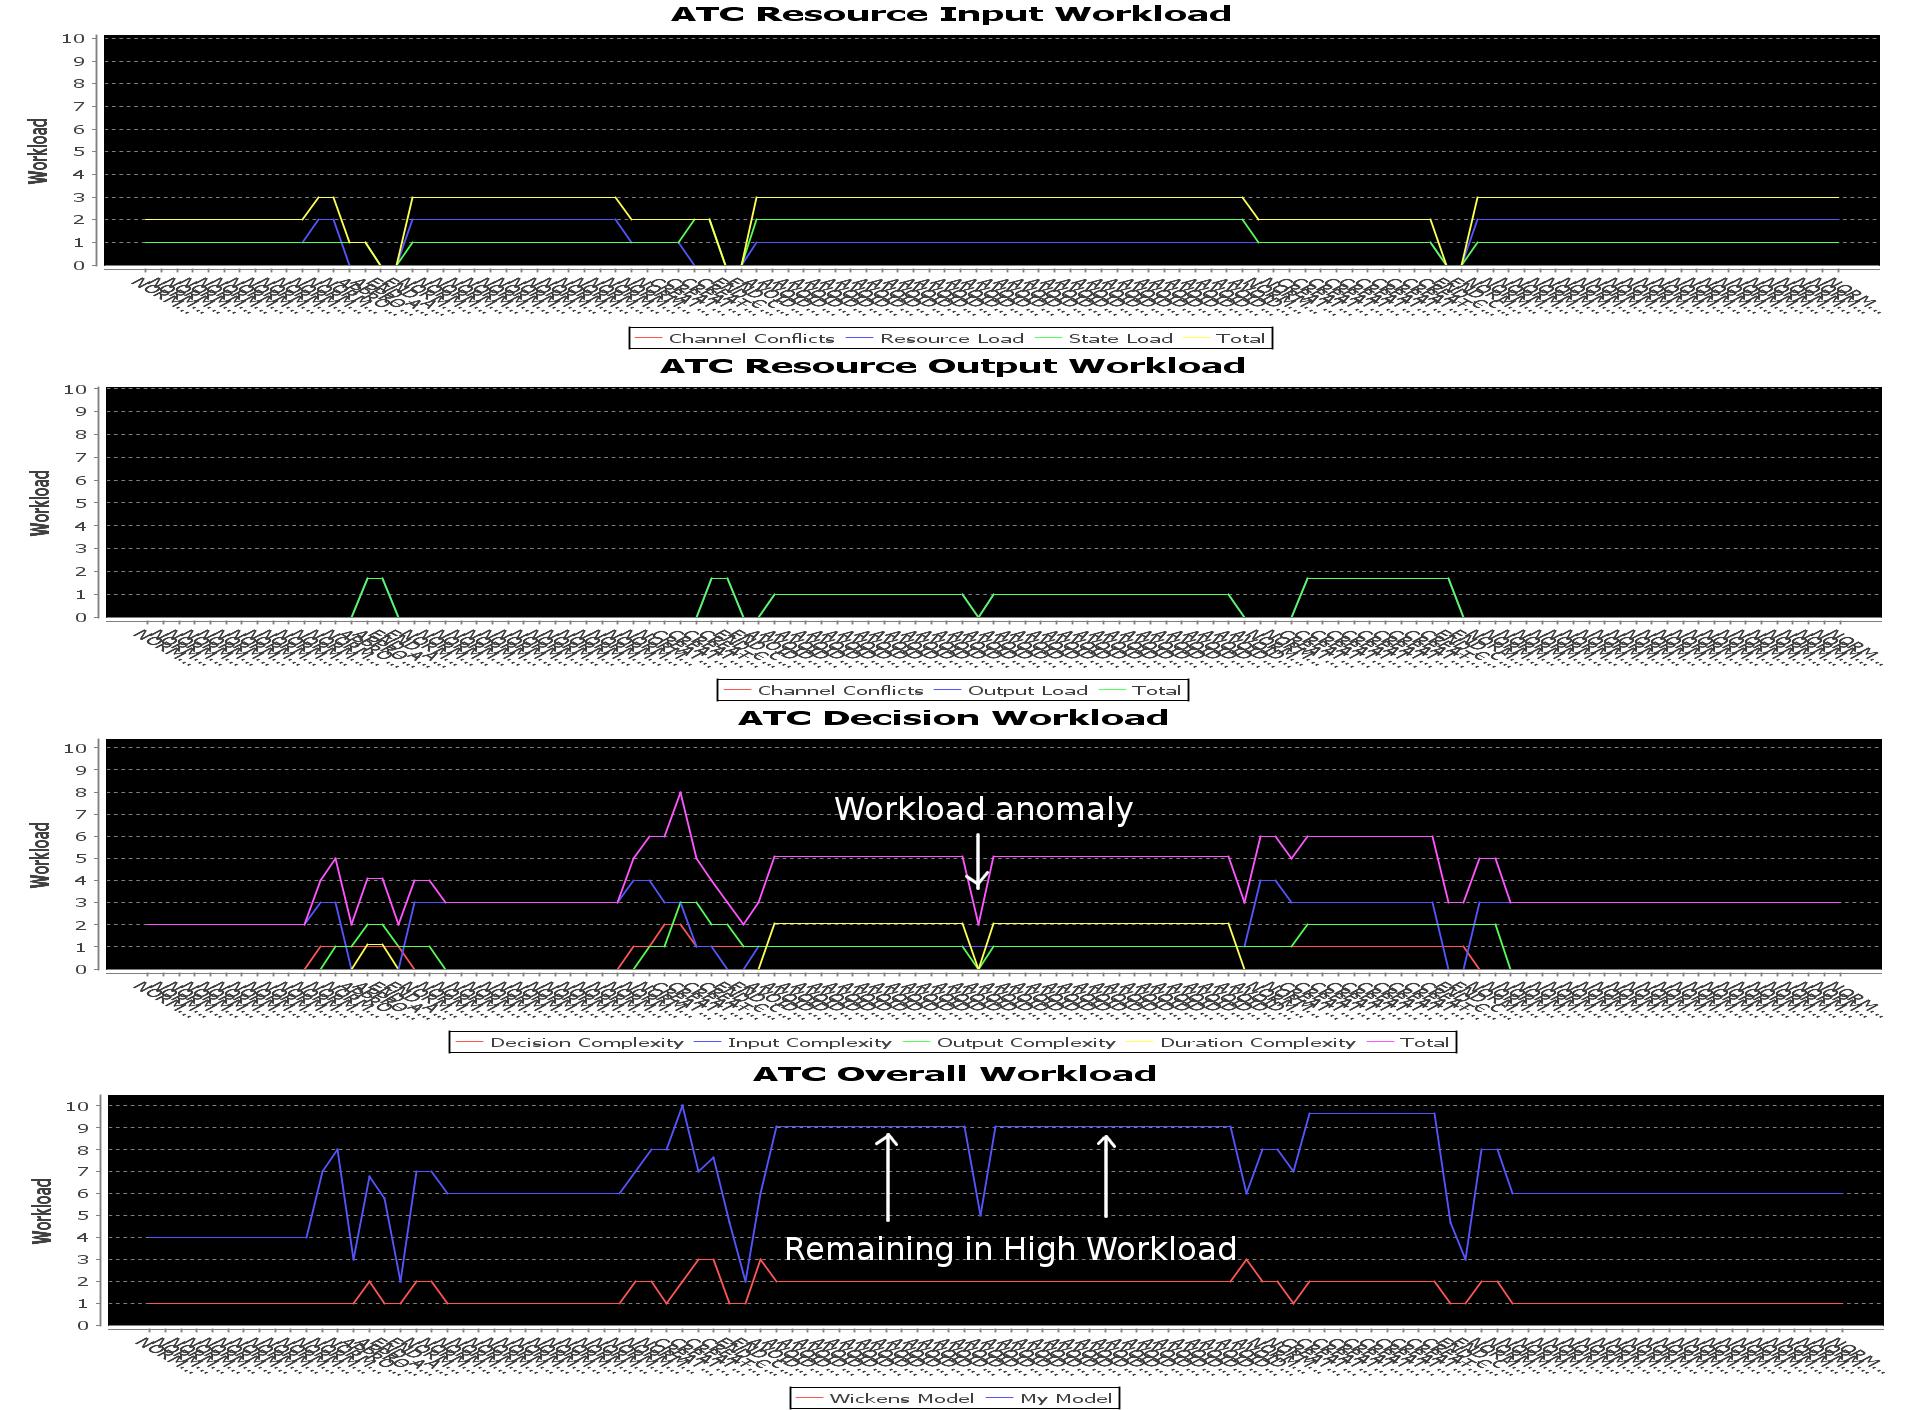
\includegraphics[width=\textwidth,height=\textheight]{UAS_in_NAS_manual_emergency_notam_ATC.png}
\caption{ATC: Manually Avoided Emergency NOTAM}
\label{fig:atc_manual}
\end{center}
\end{figure}

\begin{figure}[p]
\begin{center}
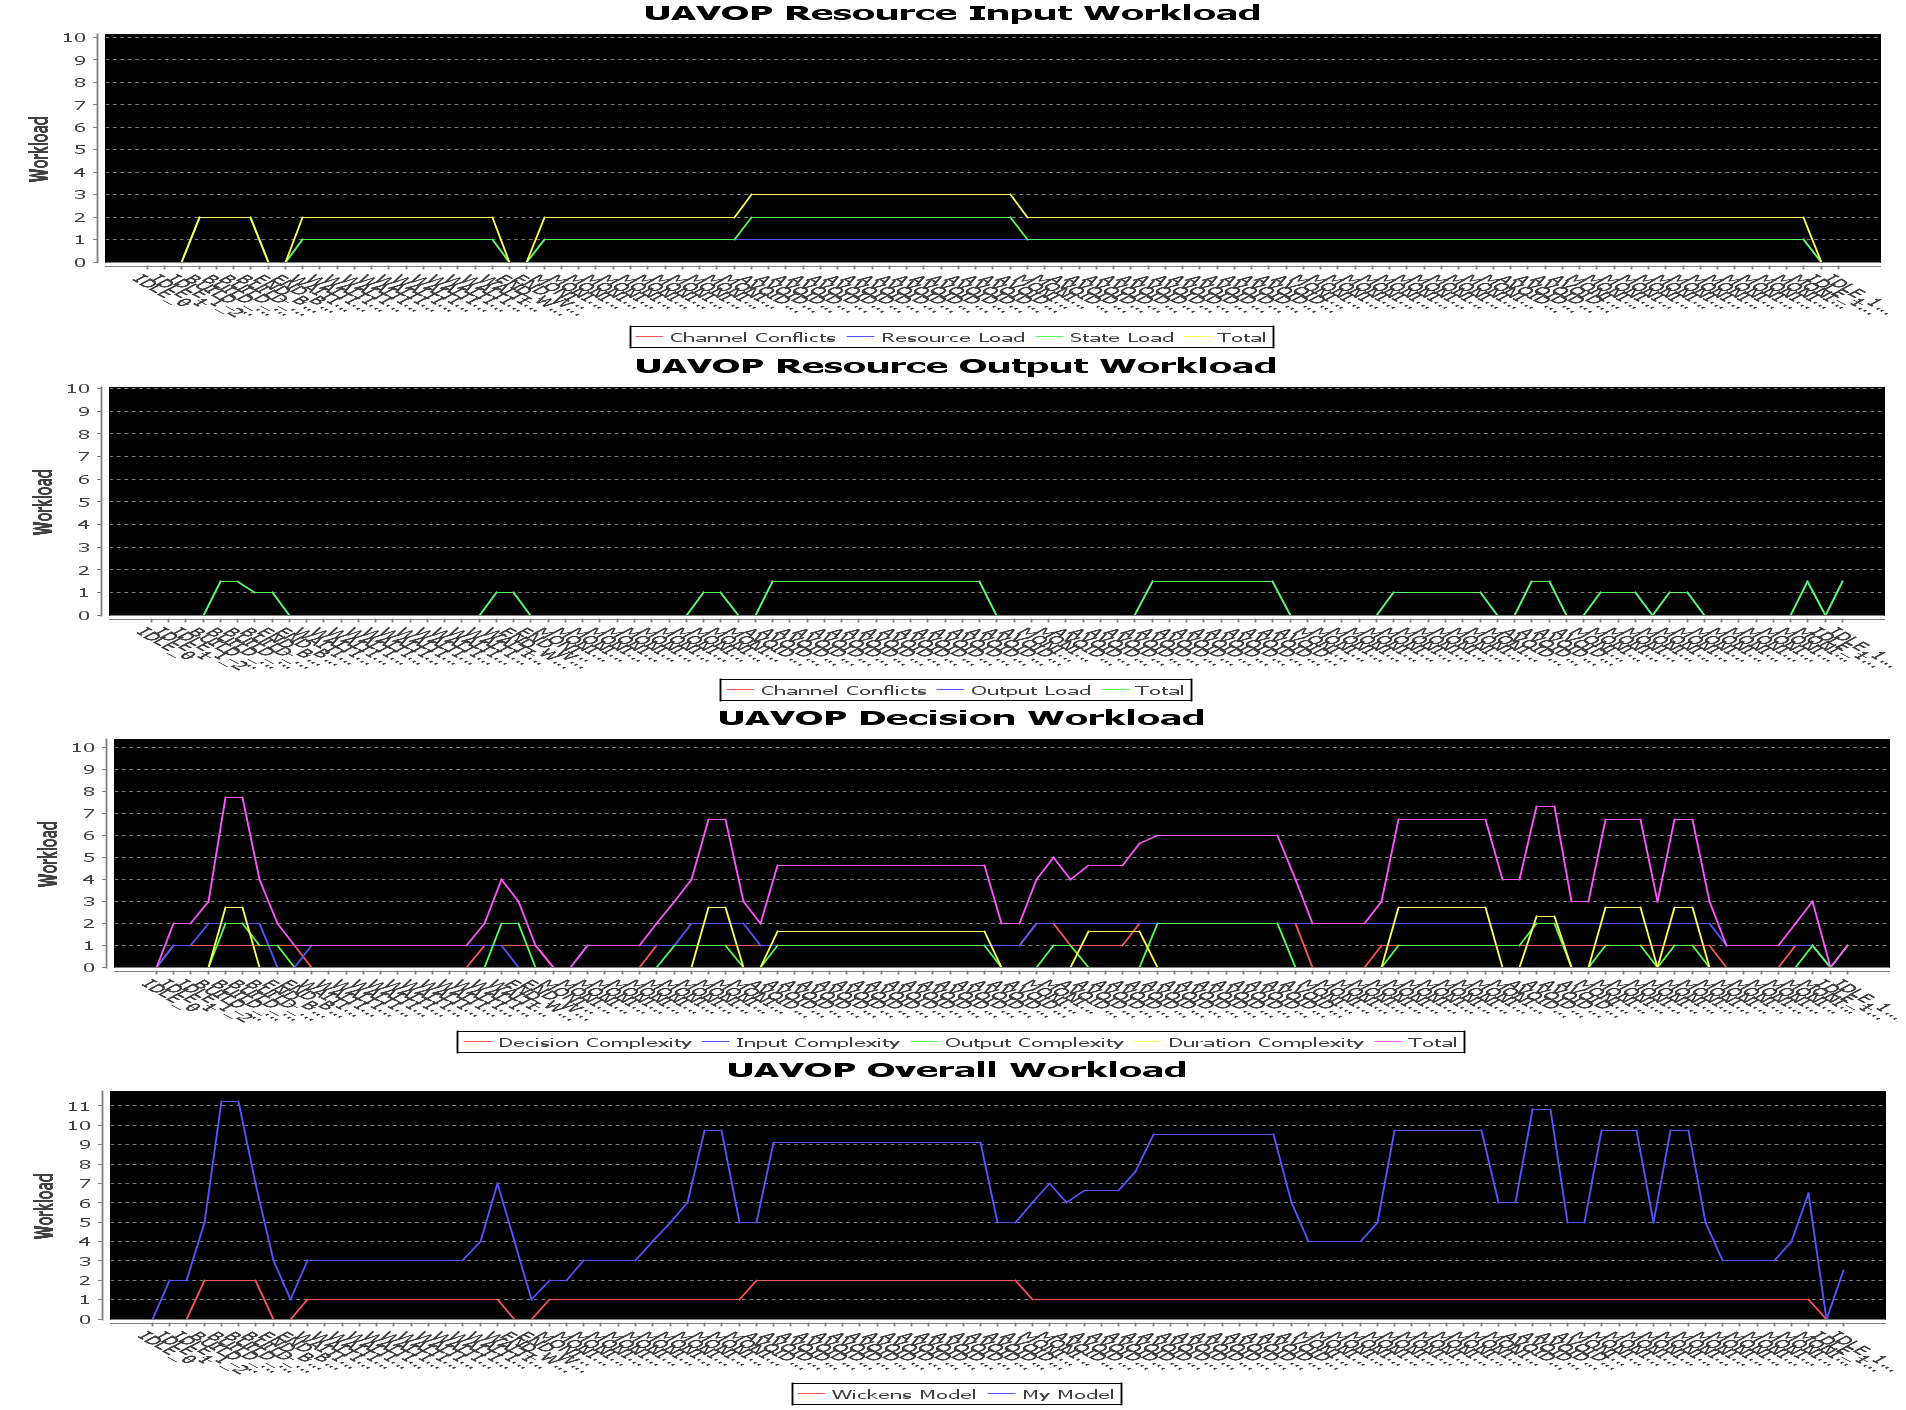
\includegraphics[width=\textwidth,height=\textheight]{UAS_in_NAS_auto_emergency_notam_UAVOP.png}
\caption{UAV Operator: Auto Avoid Emergency NOTAM}
\label{fig:uavop_auto}
\end{center}
\end{figure}

\begin{figure}[p]
\begin{center}
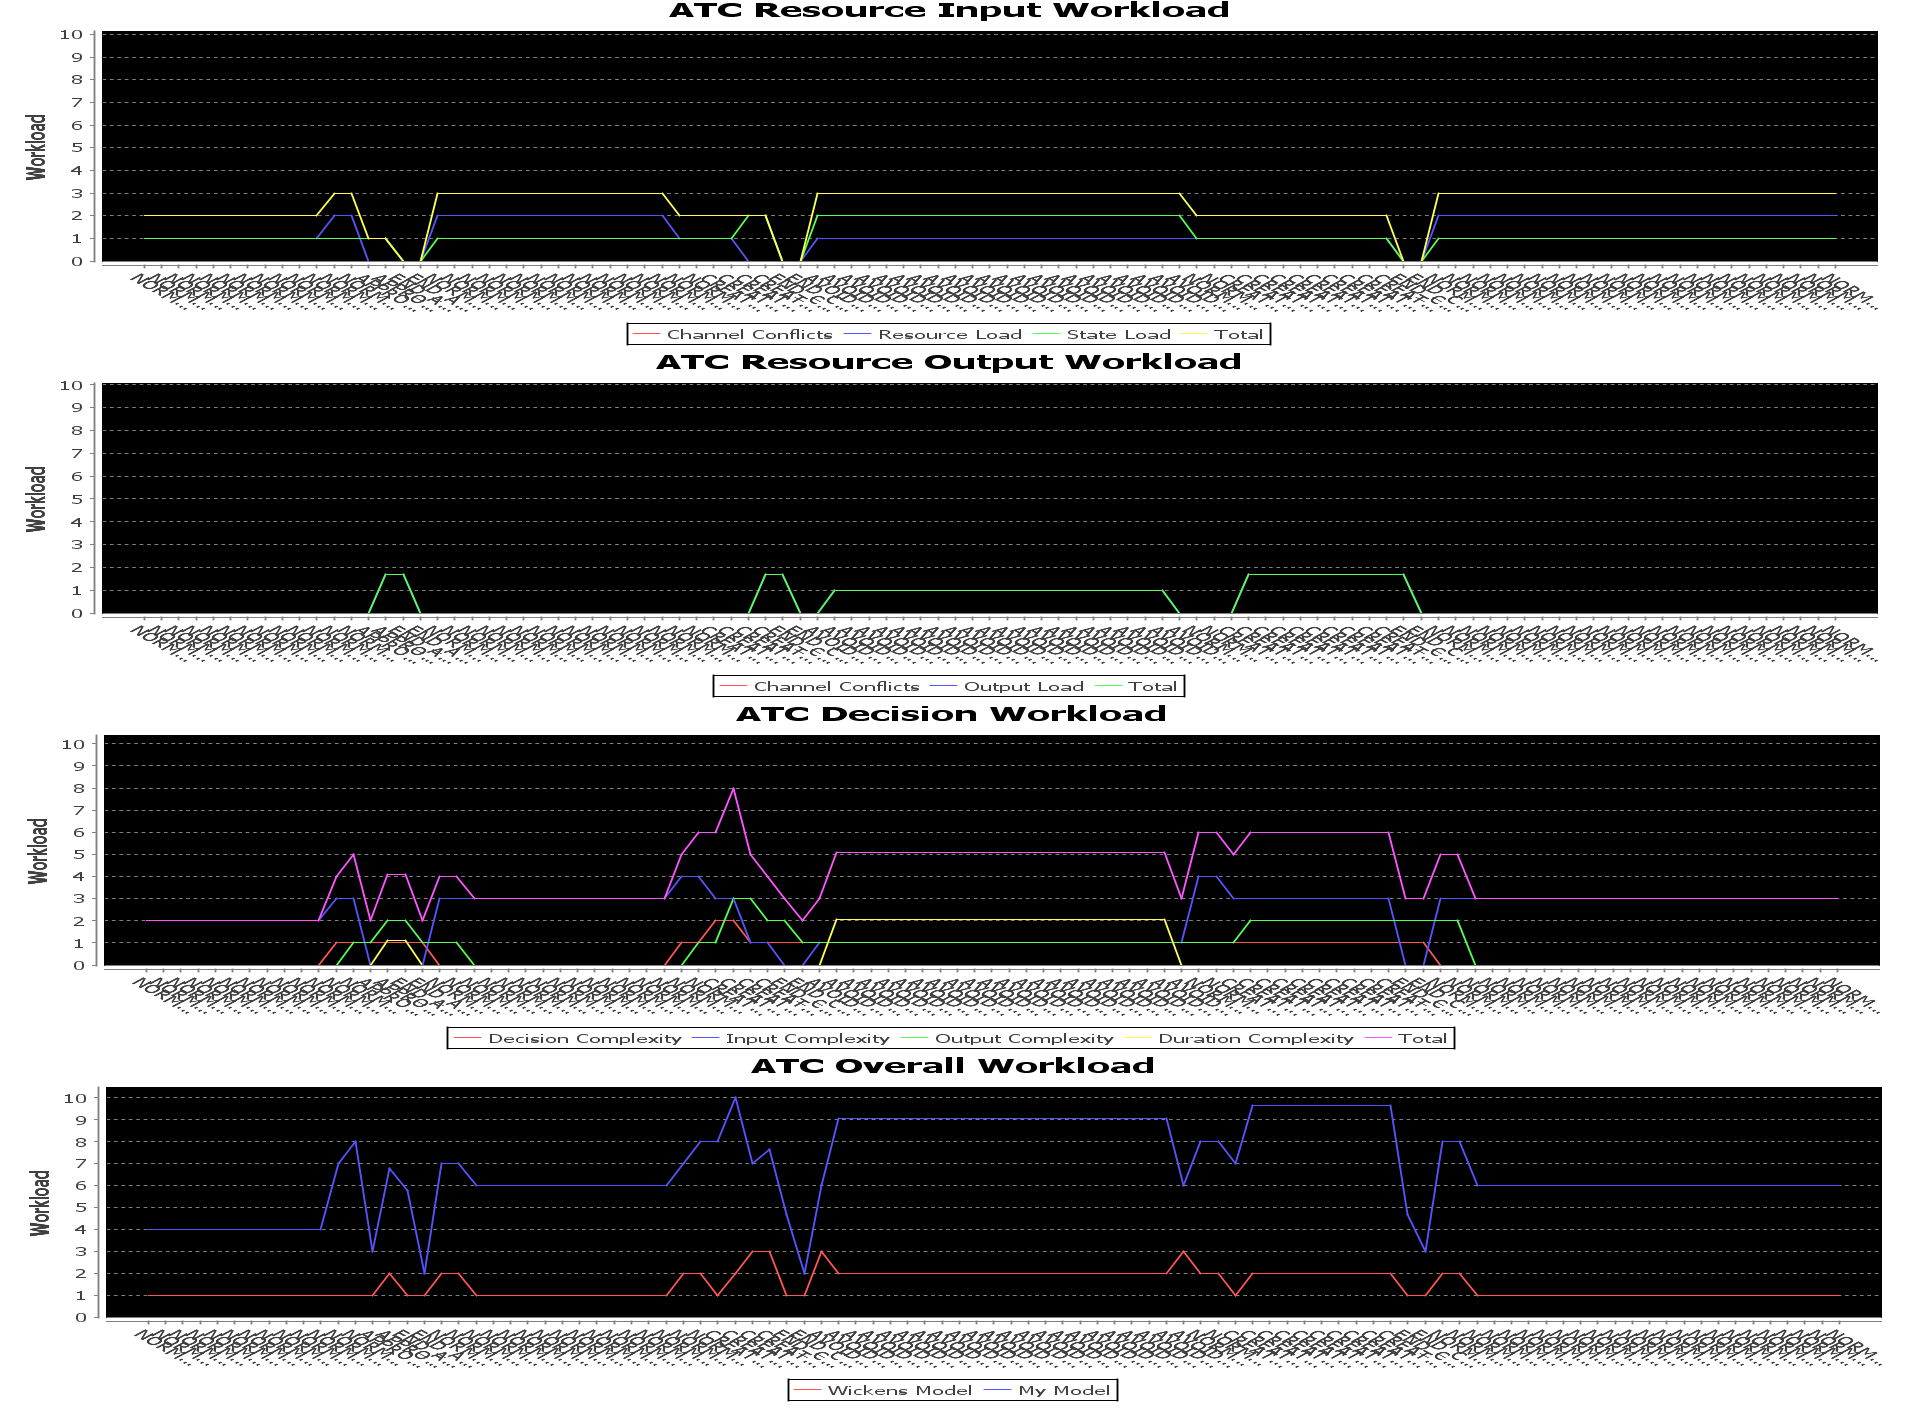
\includegraphics[width=\textwidth,height=\textheight]{UAS_in_NAS_auto_emergency_notam_ATC.png}
\caption{ATC: Auto Avoid Emergency NOTAM}
\label{fig:atc_auto}
\end{center}
\end{figure}

\begin{figure}[p]
\begin{center}
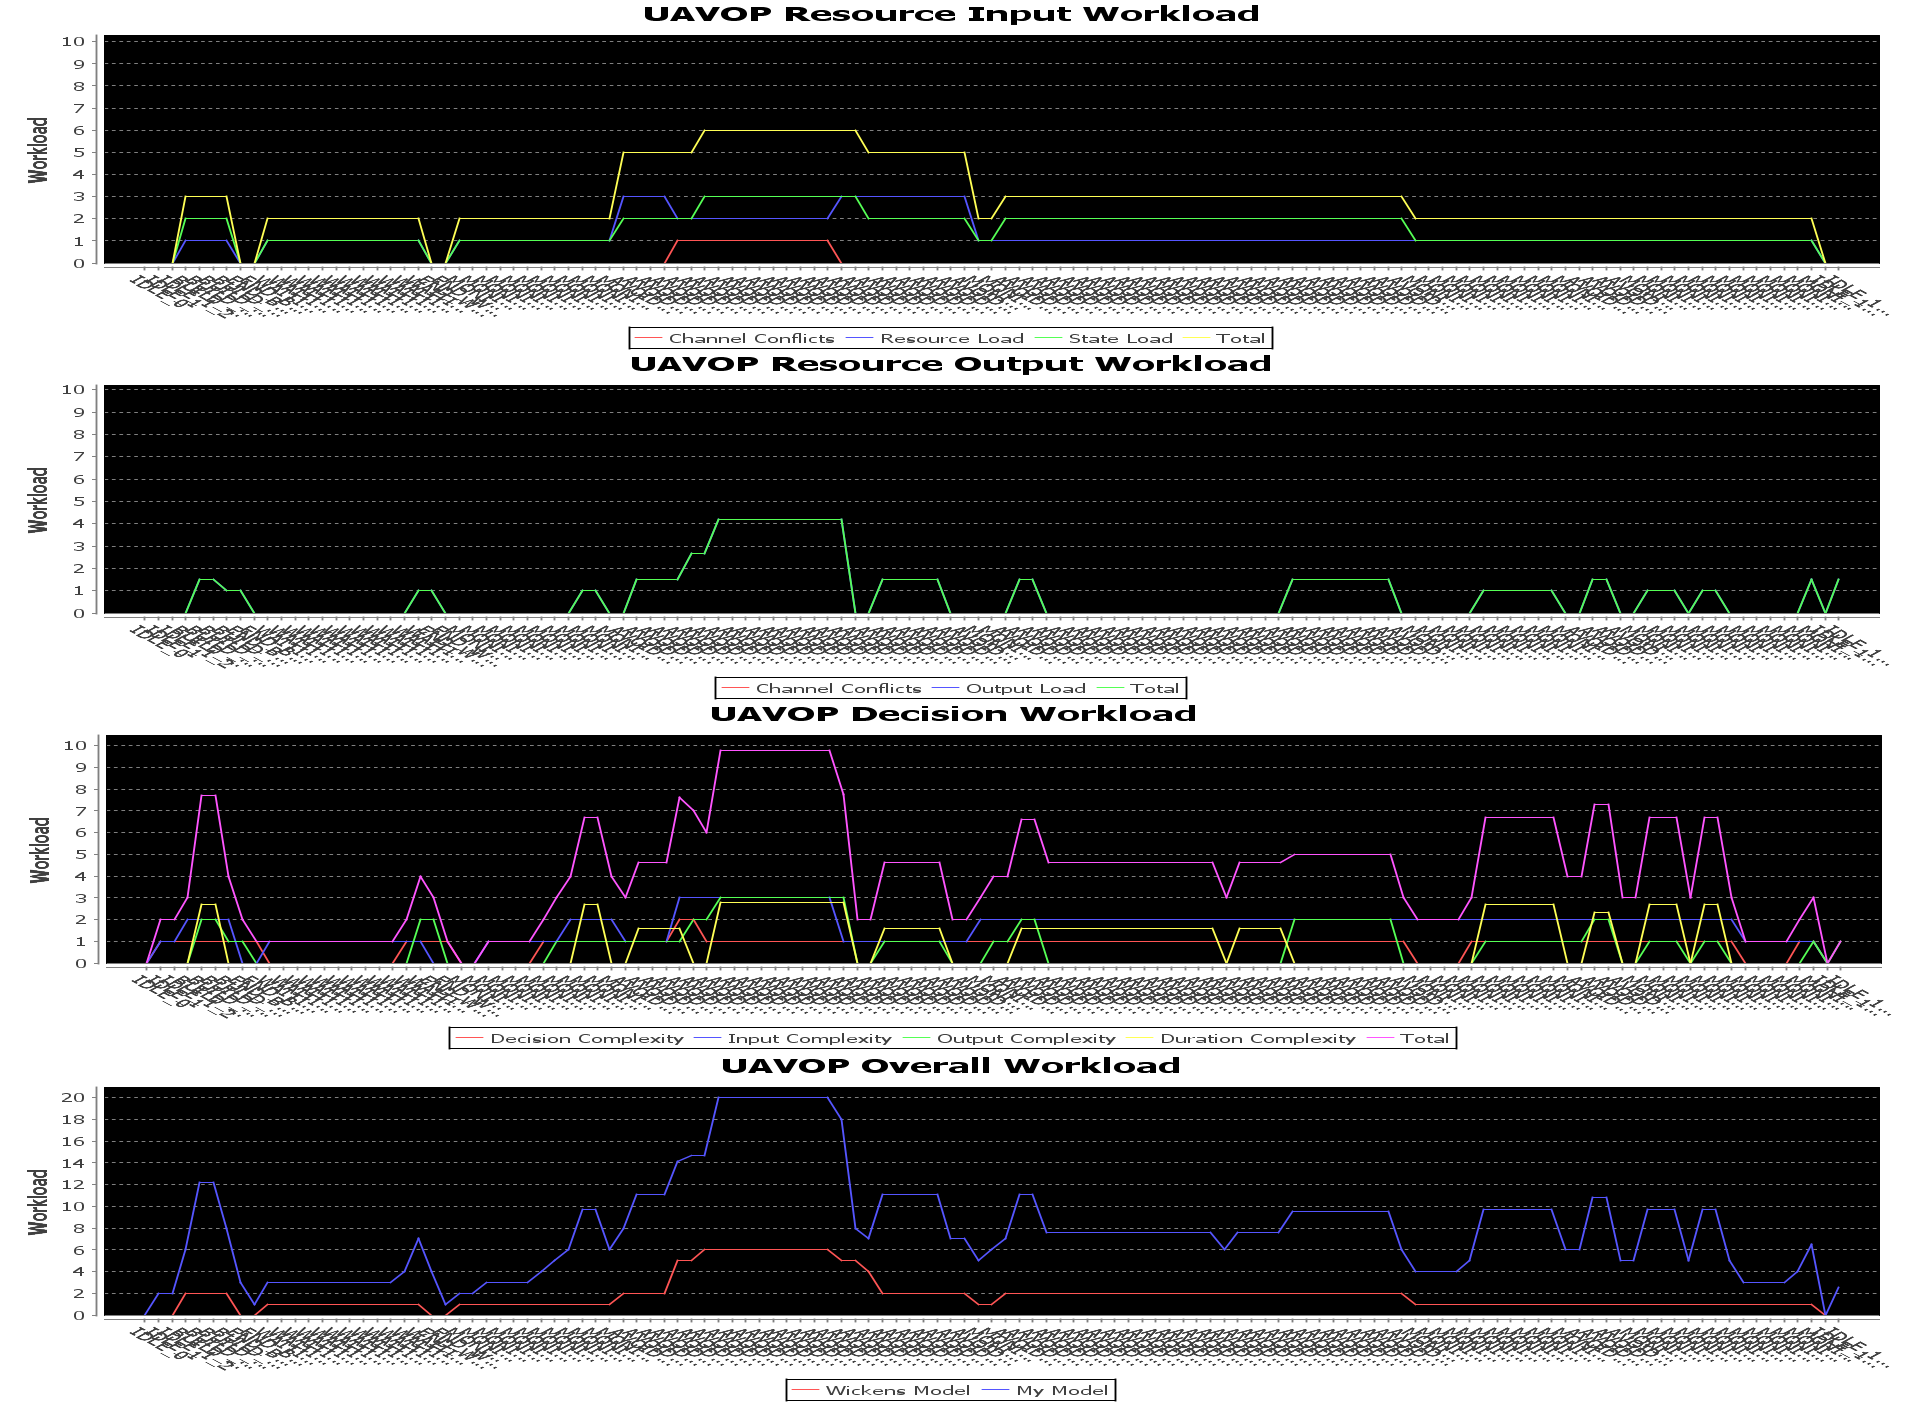
\includegraphics[width=\textwidth,height=\textheight]{UAS_in_NAS_channel_conflict_UAVOP.png}
\caption{UAVOP: Auto Avoid Emergency NOTAM w/ Interuption}
\label{fig:uavop_conflict}
\end{center}
\end{figure}
